\documentclass[12pt, a4paper, oneside]{article}	% {article|letter|report}

\newcommand{\studentPreambleFolder}{C:/Users/DGL/dotfiles/LaTeX}
\input{\studentPreambleFolder/preamble}

\fancyheadoffset[R]{0.05cm} %так можно регулировать ширину колонтитула
\pagestyle{fancy}
\fancyhead[L]{\small Подготовлено для 10 класса LancmanSchool, 13.01.21}
\fancyhead[R]{\small denisov0gleb@gmail.com}

\begin{document}

\begin{enumerate}[1.] % \marginpar{Д{\slash}З}
	\item
		Фамилия

		\hrulefill

	\item
		Имя

		\hrulefill

	\item
		Что нравится в химии?

		\hrulefill

		\hrulefill

	\item
		Что \textbf{не} нравится в химии?

		\hrulefill

		\hrulefill

	\item
		Какие есть хобби и интересы?

		\hrulefill

		\hrulefill

	\item
		Изобразите структурную формулу 3-метилбутена-1.

		\vspace{5cm}

	\item
		Назовите следующее соединение:

		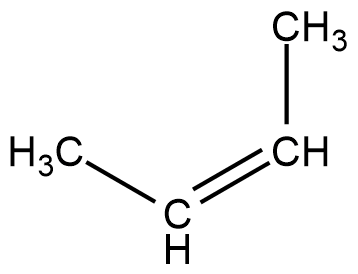
\includegraphics[scale=0.5]{10_13.01.21.png}

		\hrulefill

		\hrulefill

	\item
		Вычислите молекулярную массу вещества из предыдущего номера:

		\hrulefill

		\hrulefill

\end{enumerate}

\end{document}
